% ****** Start of file aipsamp.tex ******
%
%   This file is part of the AIP files in the AIP distribution for REVTeX 4.
%   Version 4.1 of REVTeX, October 2009
%
%   Copyright (c) 2009 American Institute of Physics.
%
%   See the AIP README file for restrictions and more information.
%
% TeX'ing this file requires that you have AMS-LaTeX 2.0 installed
% as well as the rest of the prerequisites for REVTeX 4.1
%
% It also requires running BibTeX. The commands are as follows:
%
%  1)  latex  aipsamp
%  2)  bibtex aipsamp
%  3)  latex  aipsamp
%  4)  latex  aipsamp
%
% Use this file as a source of example code for your aip document.
% Use the file aiptemplate.tex as a template for your document.
\documentclass[%
 aip,
 jmp,
 amsmath,
 amssymb,
%preprint,%
 reprint,%
%author-year,%
%author-numerical,%
 numerical,
 longbibliography,
]{revtex4-1}

\usepackage{graphicx}% Include figure files
\graphicspath{{images/}}
\usepackage{dcolumn}% Align table columns on decimal point
\usepackage{bm}% bold math
\usepackage{url}
\usepackage{float}
\usepackage{silence}
\usepackage{tabularx}
\usepackage{verbatimbox}
\WarningFilter{revtex4-1}{Repair the float}
%\usepackage[mathlines]{lineno}% Enable numbering of text and display math
%\linenumbers\relax % Commence numbering lines

\begin{document}

%\preprint{AIP/123-QED}

\title[Laboratory 3]{Introduction to Power Supplies} % Force line breaks with \\

\author{Kevin "Yama" Keyser}
 \email{kk8r8@mail.umck.edu}
\affiliation{ 
	University of Missouri-Kansas City
	%\\This line break forced with \textbackslash\textbackslash
}%

%\date{\today}% It is always \today, today,
             %  but any date may be explicitly specified

\begin{abstract}
In Laboratory 3, we begin our introduction to transformers, diodes, and their applications
to electronic circuits. We continue our expanding our knowledge of using oscilloscopes and
plotting two functions on the same graph in order to quantitatively compare our input
to our output, to try to understand the visual difference of what our circuit is doing
to our input voltage.
\end{abstract}

%\keywords{Operational Amplifier}%Use showkeys class option if keyword
                              %display desired
\maketitle

%\begin{quotation}
%The ``lead paragraph'' is encapsulated with the \LaTeX\ 
%\verb+quotation+ environment and is formatted as a single paragraph before the first section heading. 
%(The \verb+quotation+ environment reverts to its usual meaning after the first sectioning command.) 
%Note that numbered references are allowed in the lead paragraph.
%
%The lead paragraph will only be found in an article being prepared for the journal \textit{Chaos}.
%\end{quotation}

\section{Background}

For Laboratory 3, the main background information we need to understand will be how to
use an oscilloscope, to know how to properly ground and not short our circuit, and
what direction our diodes should be placed in our circuit.

\section{Procedure}

The procedures for Laboratory 3 will be attached as a separate sheet of paper to the back
of the laboratory write up.

\section{Presentation of Data}

	\subsection{3-1: Transformer Output Voltage Measurements}
	
	No tabular data. All information will be presented in the Discussion section.

	\subsection{3-2: Diodes}
	
	\begin{tabularx}{0.45\textwidth}[t]{| X | X |}
	\hline
	\multicolumn{2}{|c|}{Channel 1}\\
	\hline
		\multicolumn{1}{|c|}{RMS (V)} & 
		\multicolumn{1}{c|}{Peak-to-Peak (V)} \\ 
	\hline	
	1.549 & 4.40 \\ \hline
	\multicolumn{2}{|c|}{Channel 2}\\
	\hline
		\multicolumn{1}{|c|}{RMS (V)} & 
		\multicolumn{1}{c|}{Peak-to-Peak (V)} \\ 
	\hline
	0.4573 & 1.340 \\ \hline	
	\end{tabularx}
	
	\subsection{3-3: Half-Wave Rectified Power Supply}
	
	\begin{figure}[H]
	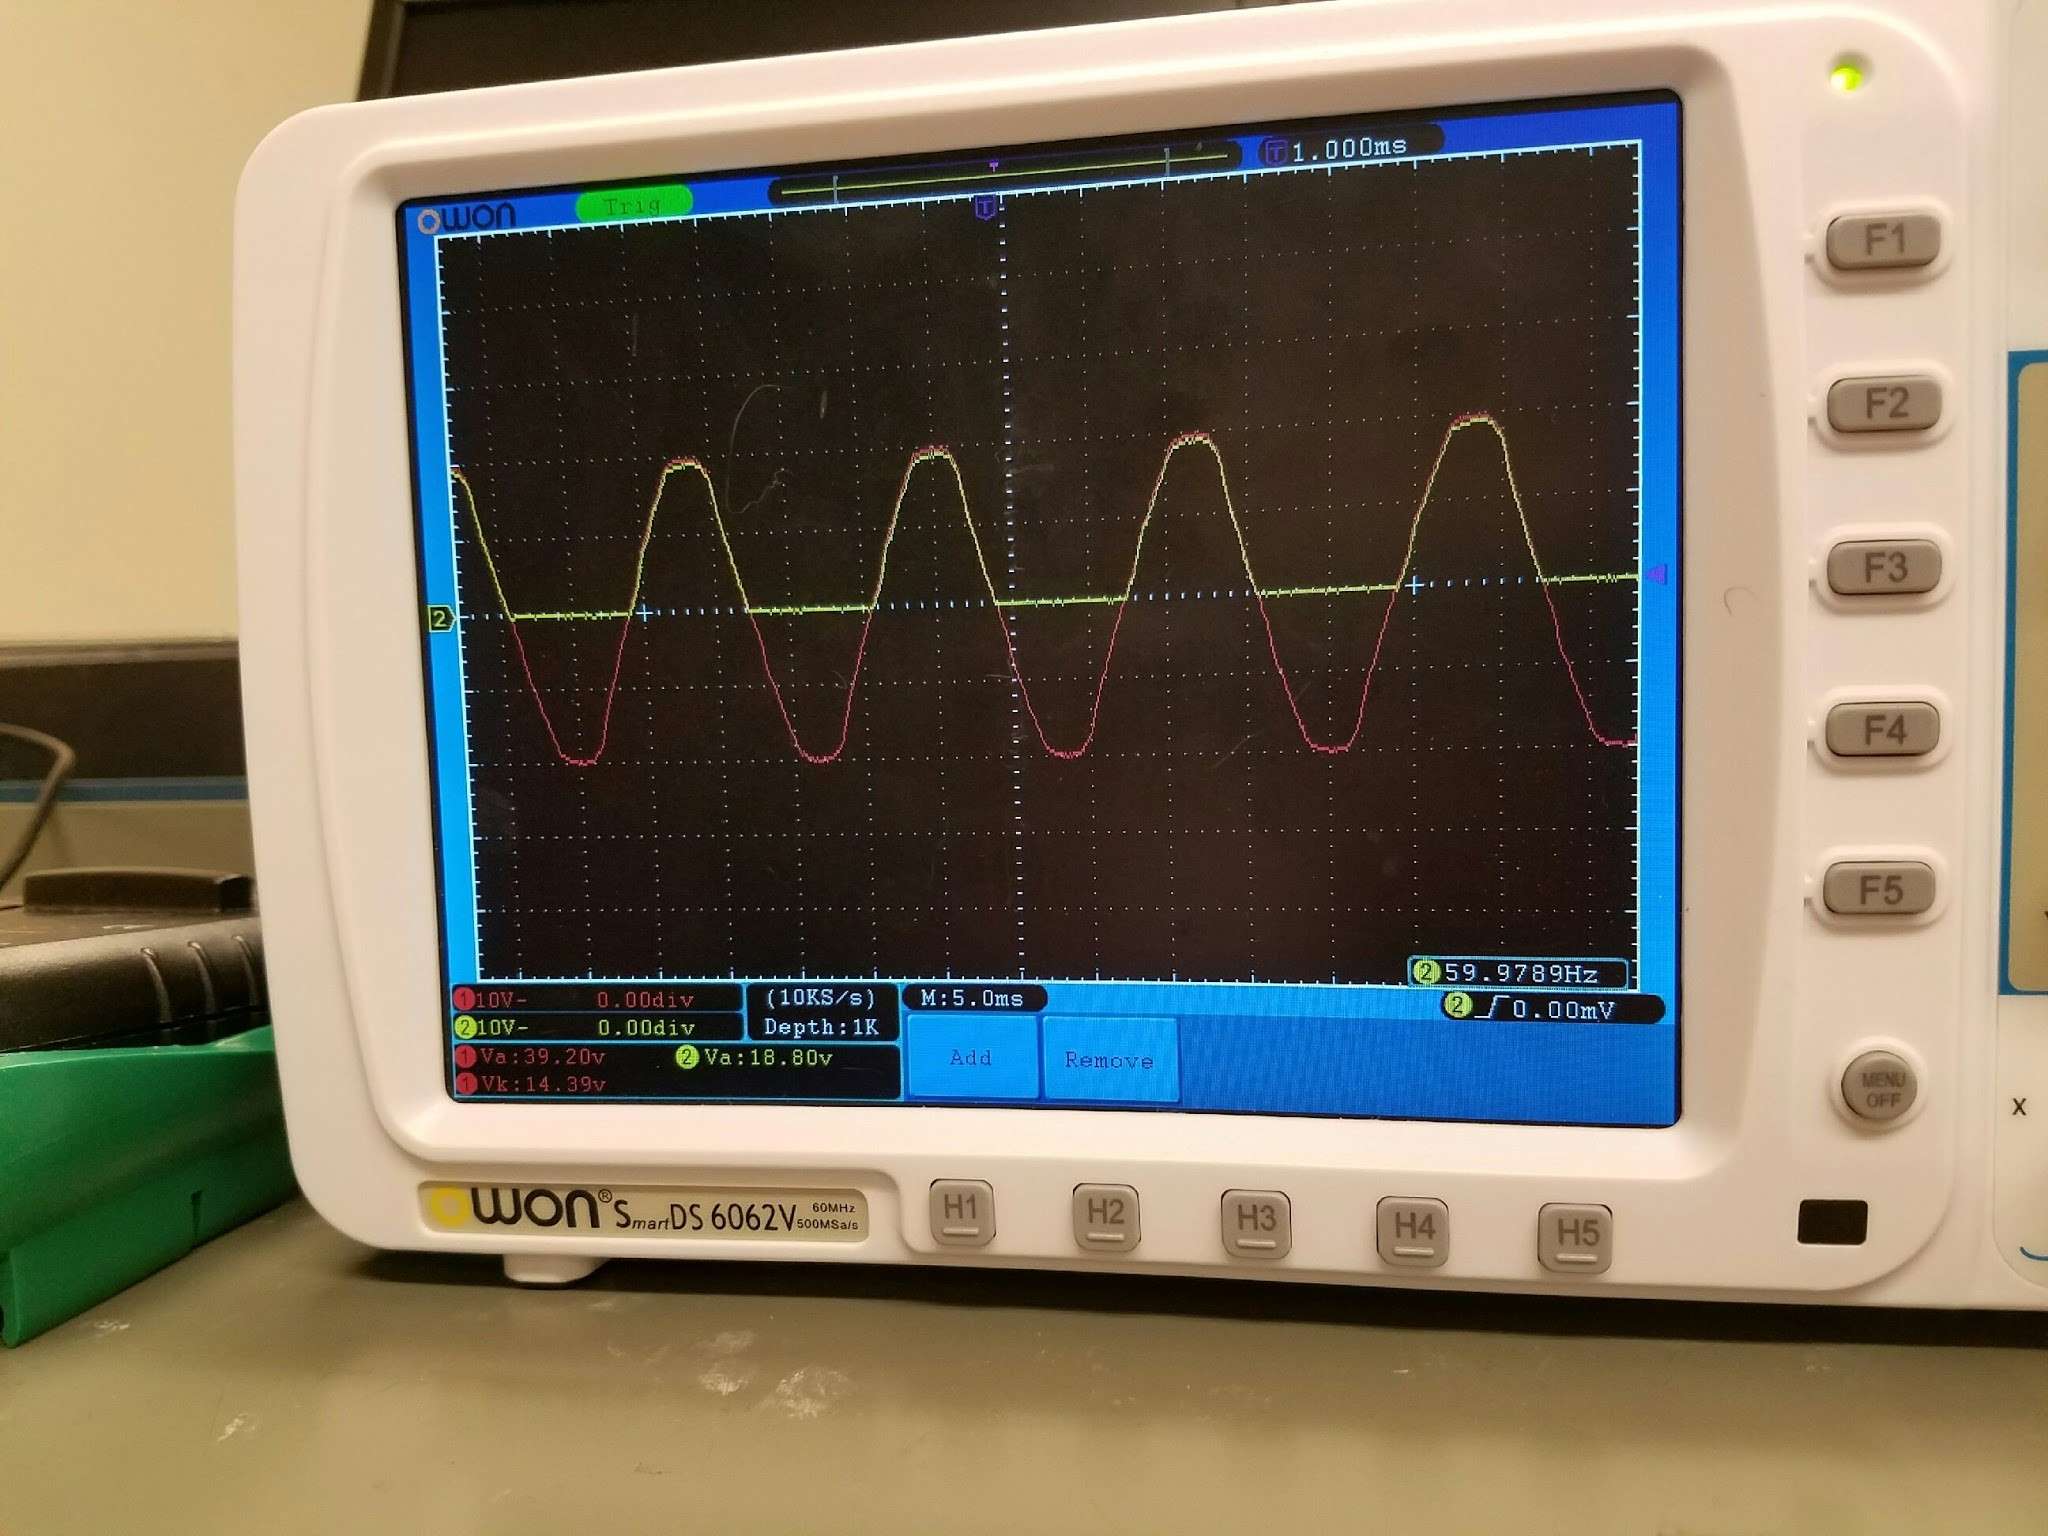
\includegraphics[width=\columnwidth]{HalfWaveRect.eps}
	\caption{Input and Output plot of a half-wave rectifier.}
	\end{figure}
	
	\begin{figure}[H]
	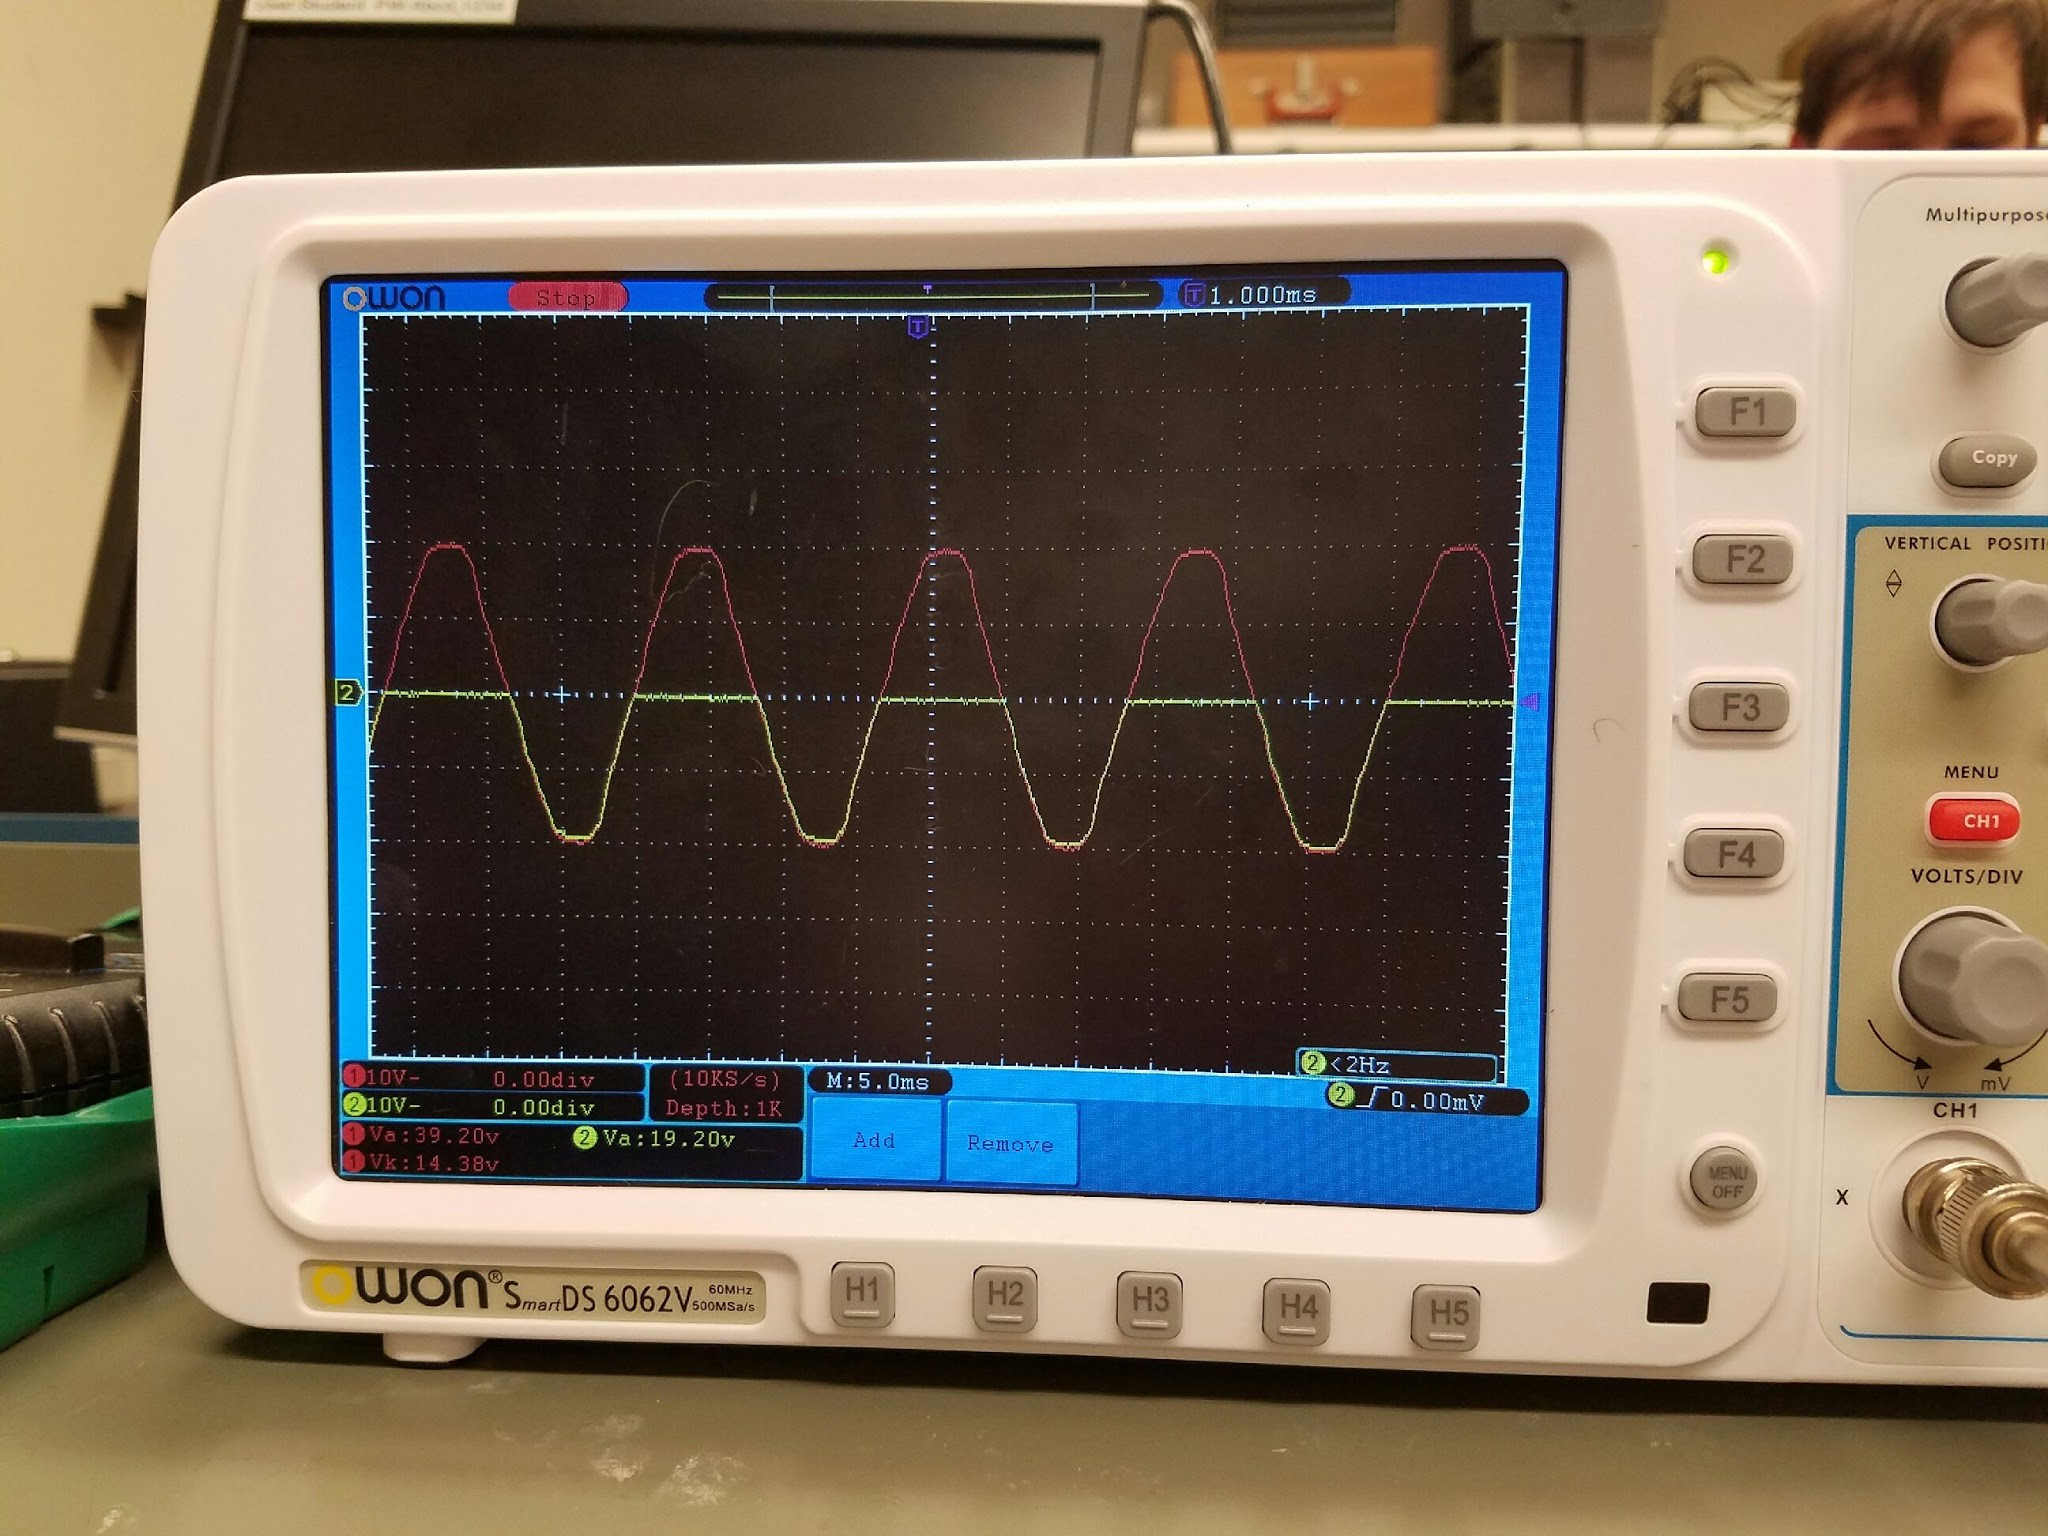
\includegraphics[width=\columnwidth]{InverseHalfWaveRect.eps}
	\caption{Input and Output plot of a half-wave rectifier, where we insert
	the diode in with a reverse bias.}
	\end{figure}	
	
	\subsection{3-4: Full-Wave Rectified}
	
	\begin{figure}[H]
	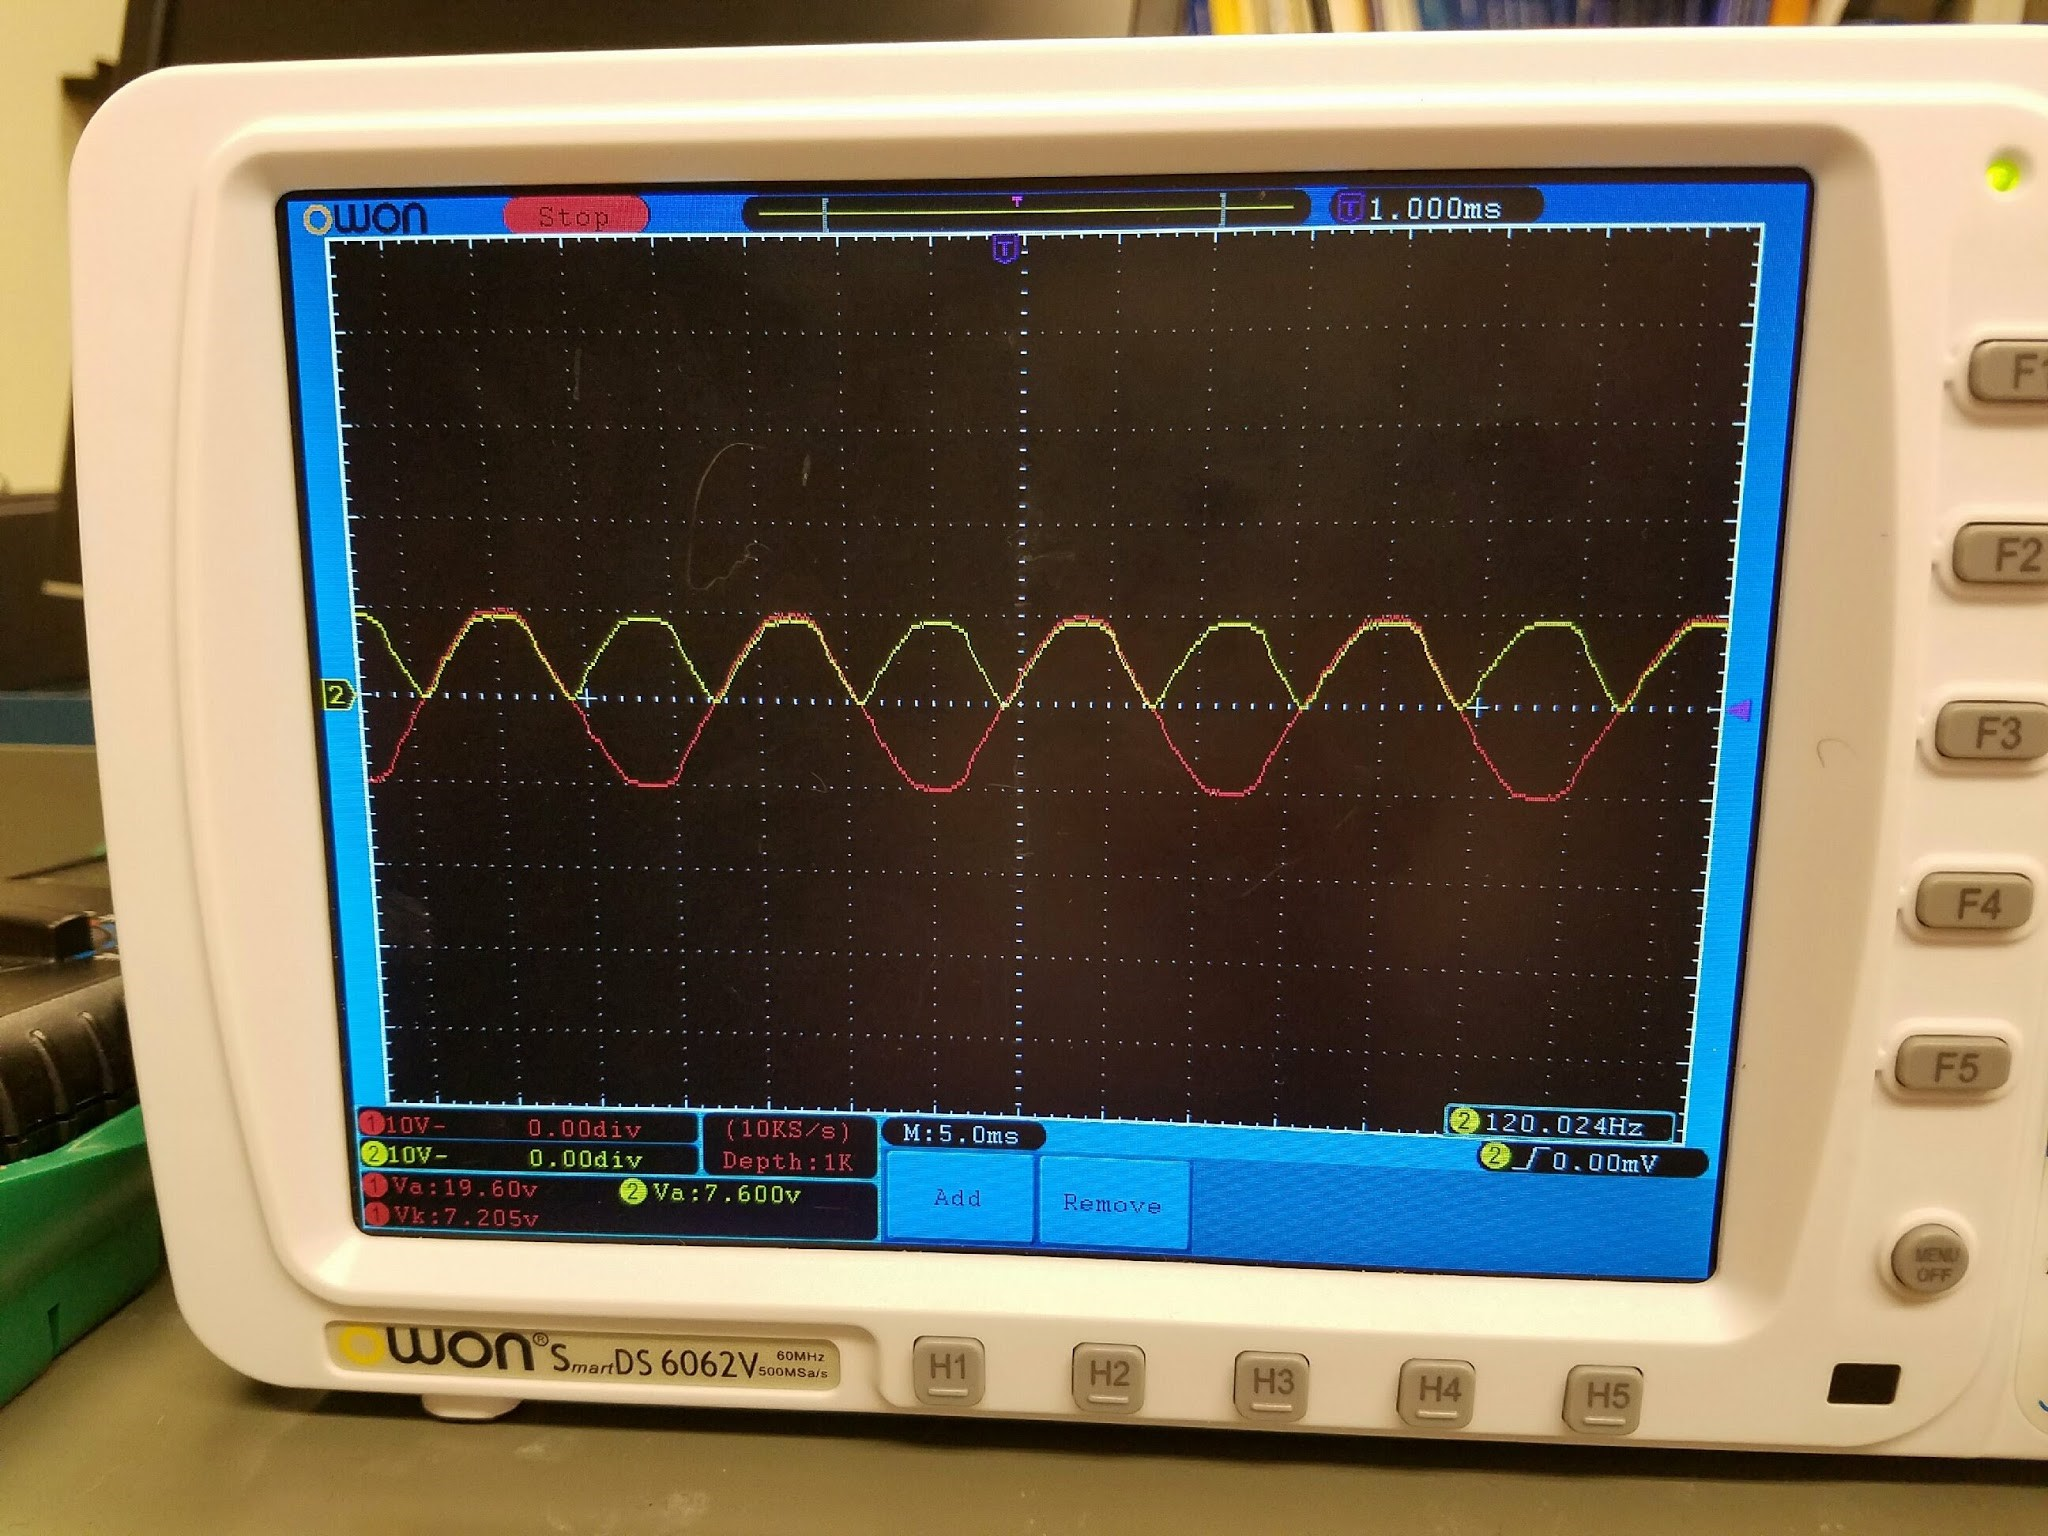
\includegraphics[width=\columnwidth]{FullWaveRect.eps}
	\caption{Input and Output plot of a full-wave rectifier.}
	\end{figure}	
	
	\subsection{3-5: Bridge Rectifier}
	
	\begin{tabularx}{0.45\textwidth}[t]{| X | X |}
	\hline
	\multicolumn{2}{|c|}{RMS}\\
	\hline
		\multicolumn{1}{|c|}{Input (V)} & 
		\multicolumn{1}{c|}{Output (V)} \\ 
	\hline	
	14.19 & 9.65 \\ \hline
	\multicolumn{2}{|c|}{Peak-to-Peak}\\
	\hline
		\multicolumn{1}{|c|}{Input (V)} & 
		\multicolumn{1}{c|}{Output (V)} \\ 
	\hline
	39.20 & 20.00 \\ \hline	
	\multicolumn{2}{|c|}{Amplitude}\\
	\hline
		\multicolumn{1}{|c|}{Input (V)} & 
		\multicolumn{1}{c|}{Output (V)} \\ 
	\hline
	38.40 & 19.60 \\ \hline		
	\end{tabularx}	
		
	\subsection{3-6: Filter Capacitors}
	
	\begin{figure}[H]
	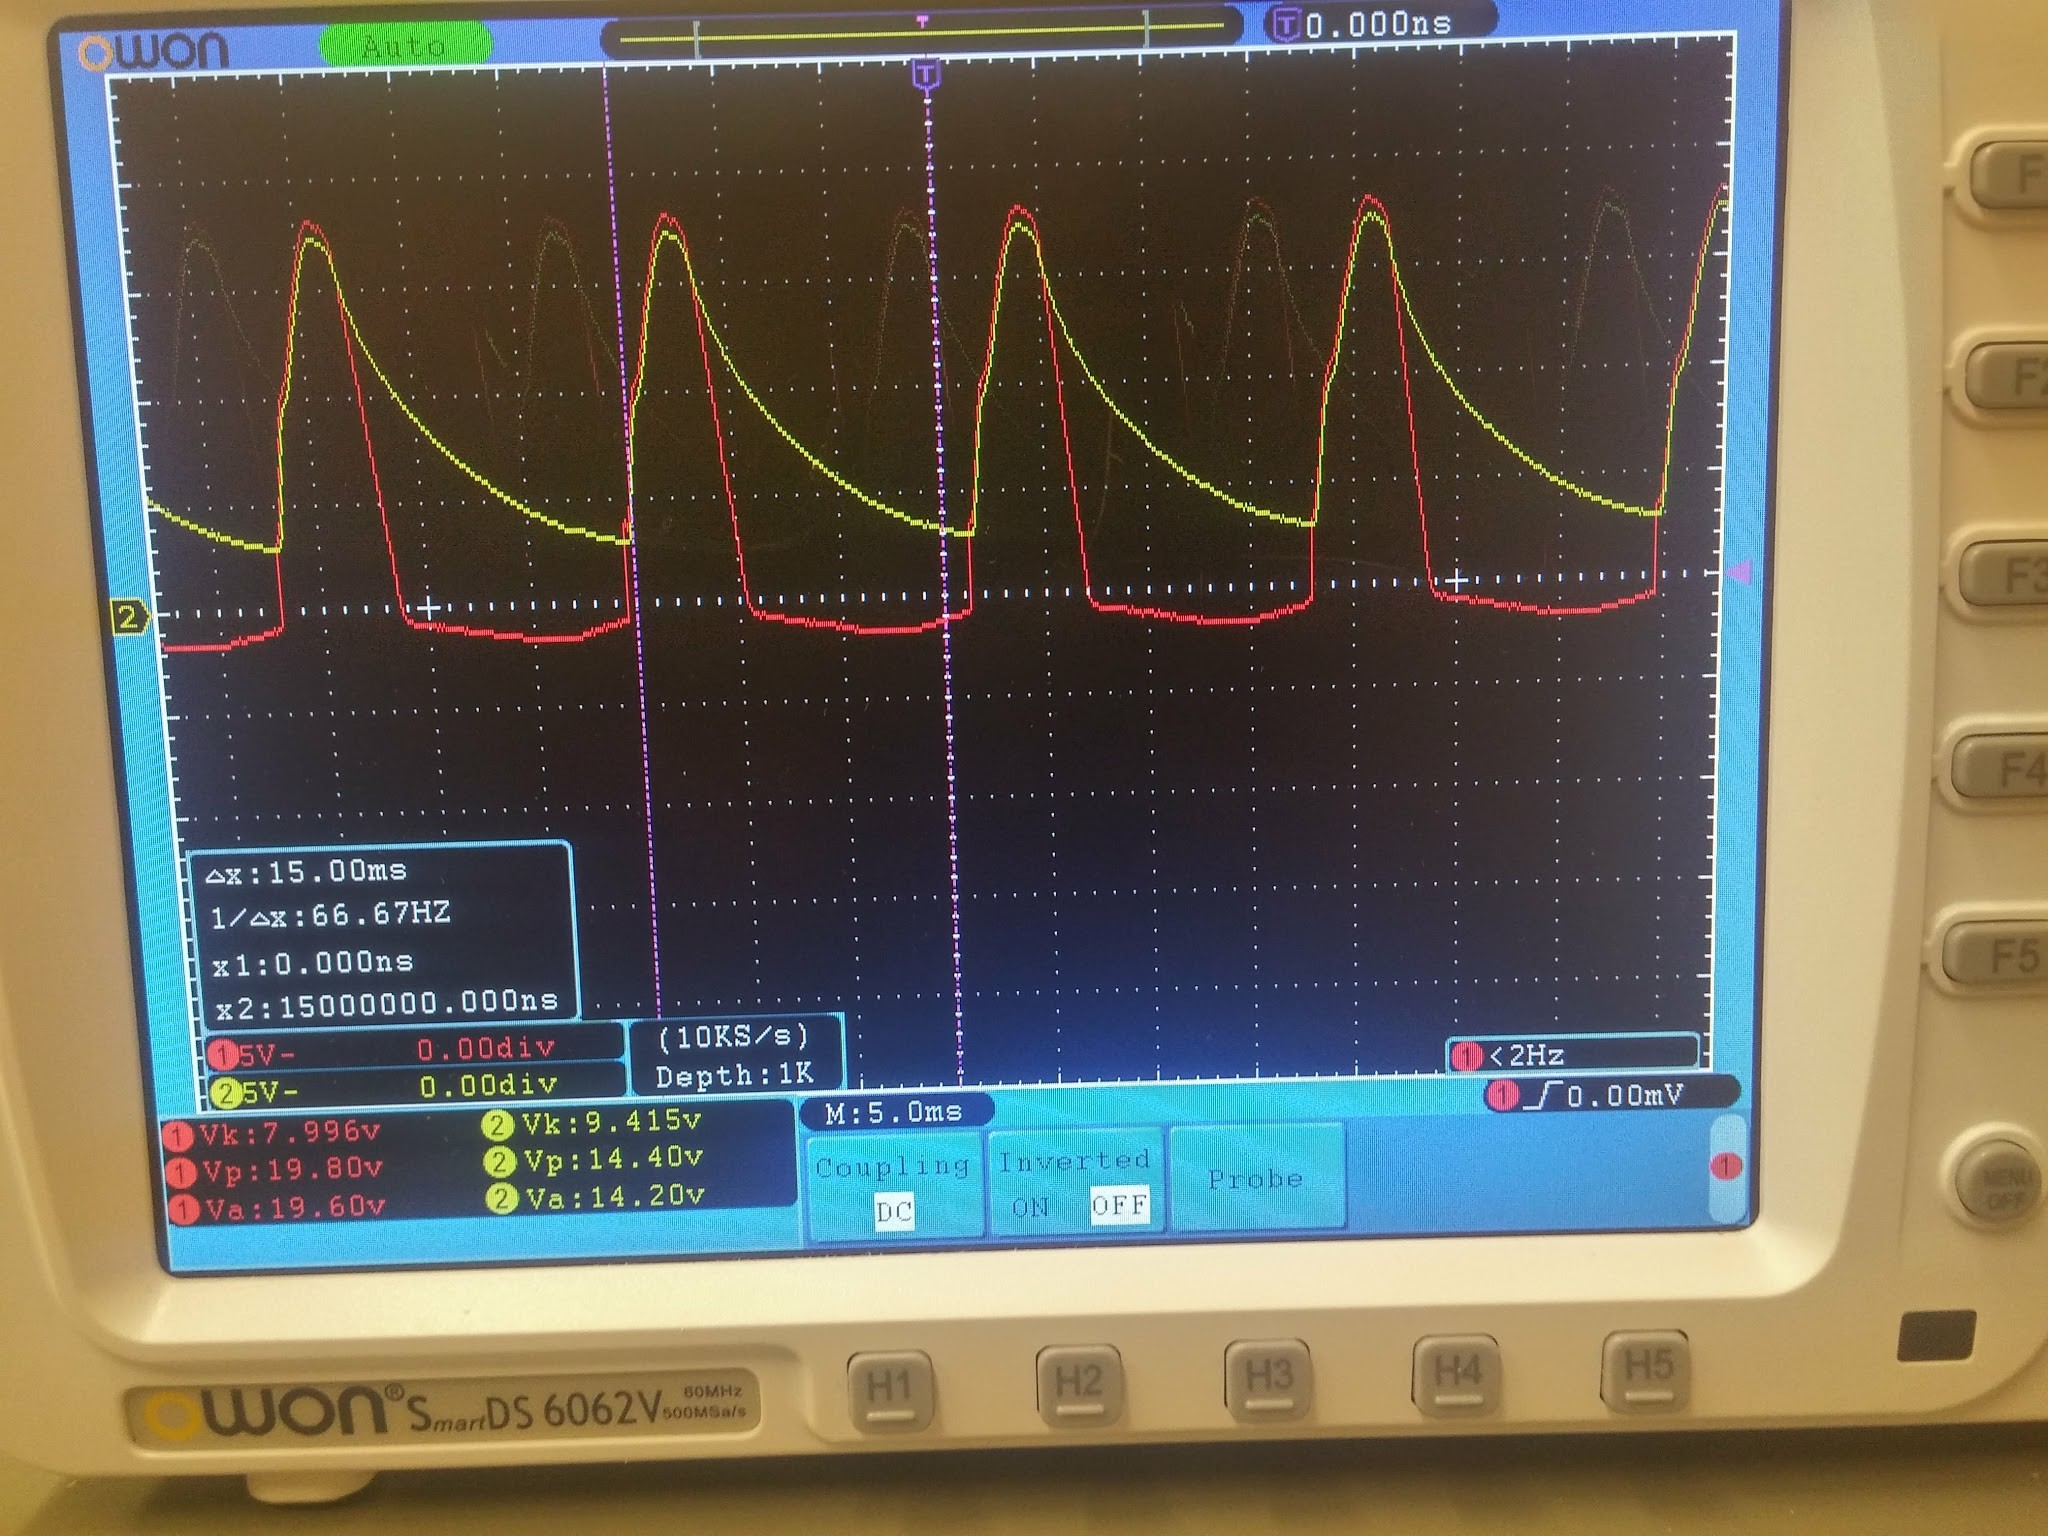
\includegraphics[width=\columnwidth]{Res200Cap10.eps}
	\caption{Input and Output of our filter capacitor circuit with a
	200$\Omega F$ resistor, and a 10$\mu F$ capacitor.}
	\end{figure}

	\begin{figure}[H]
	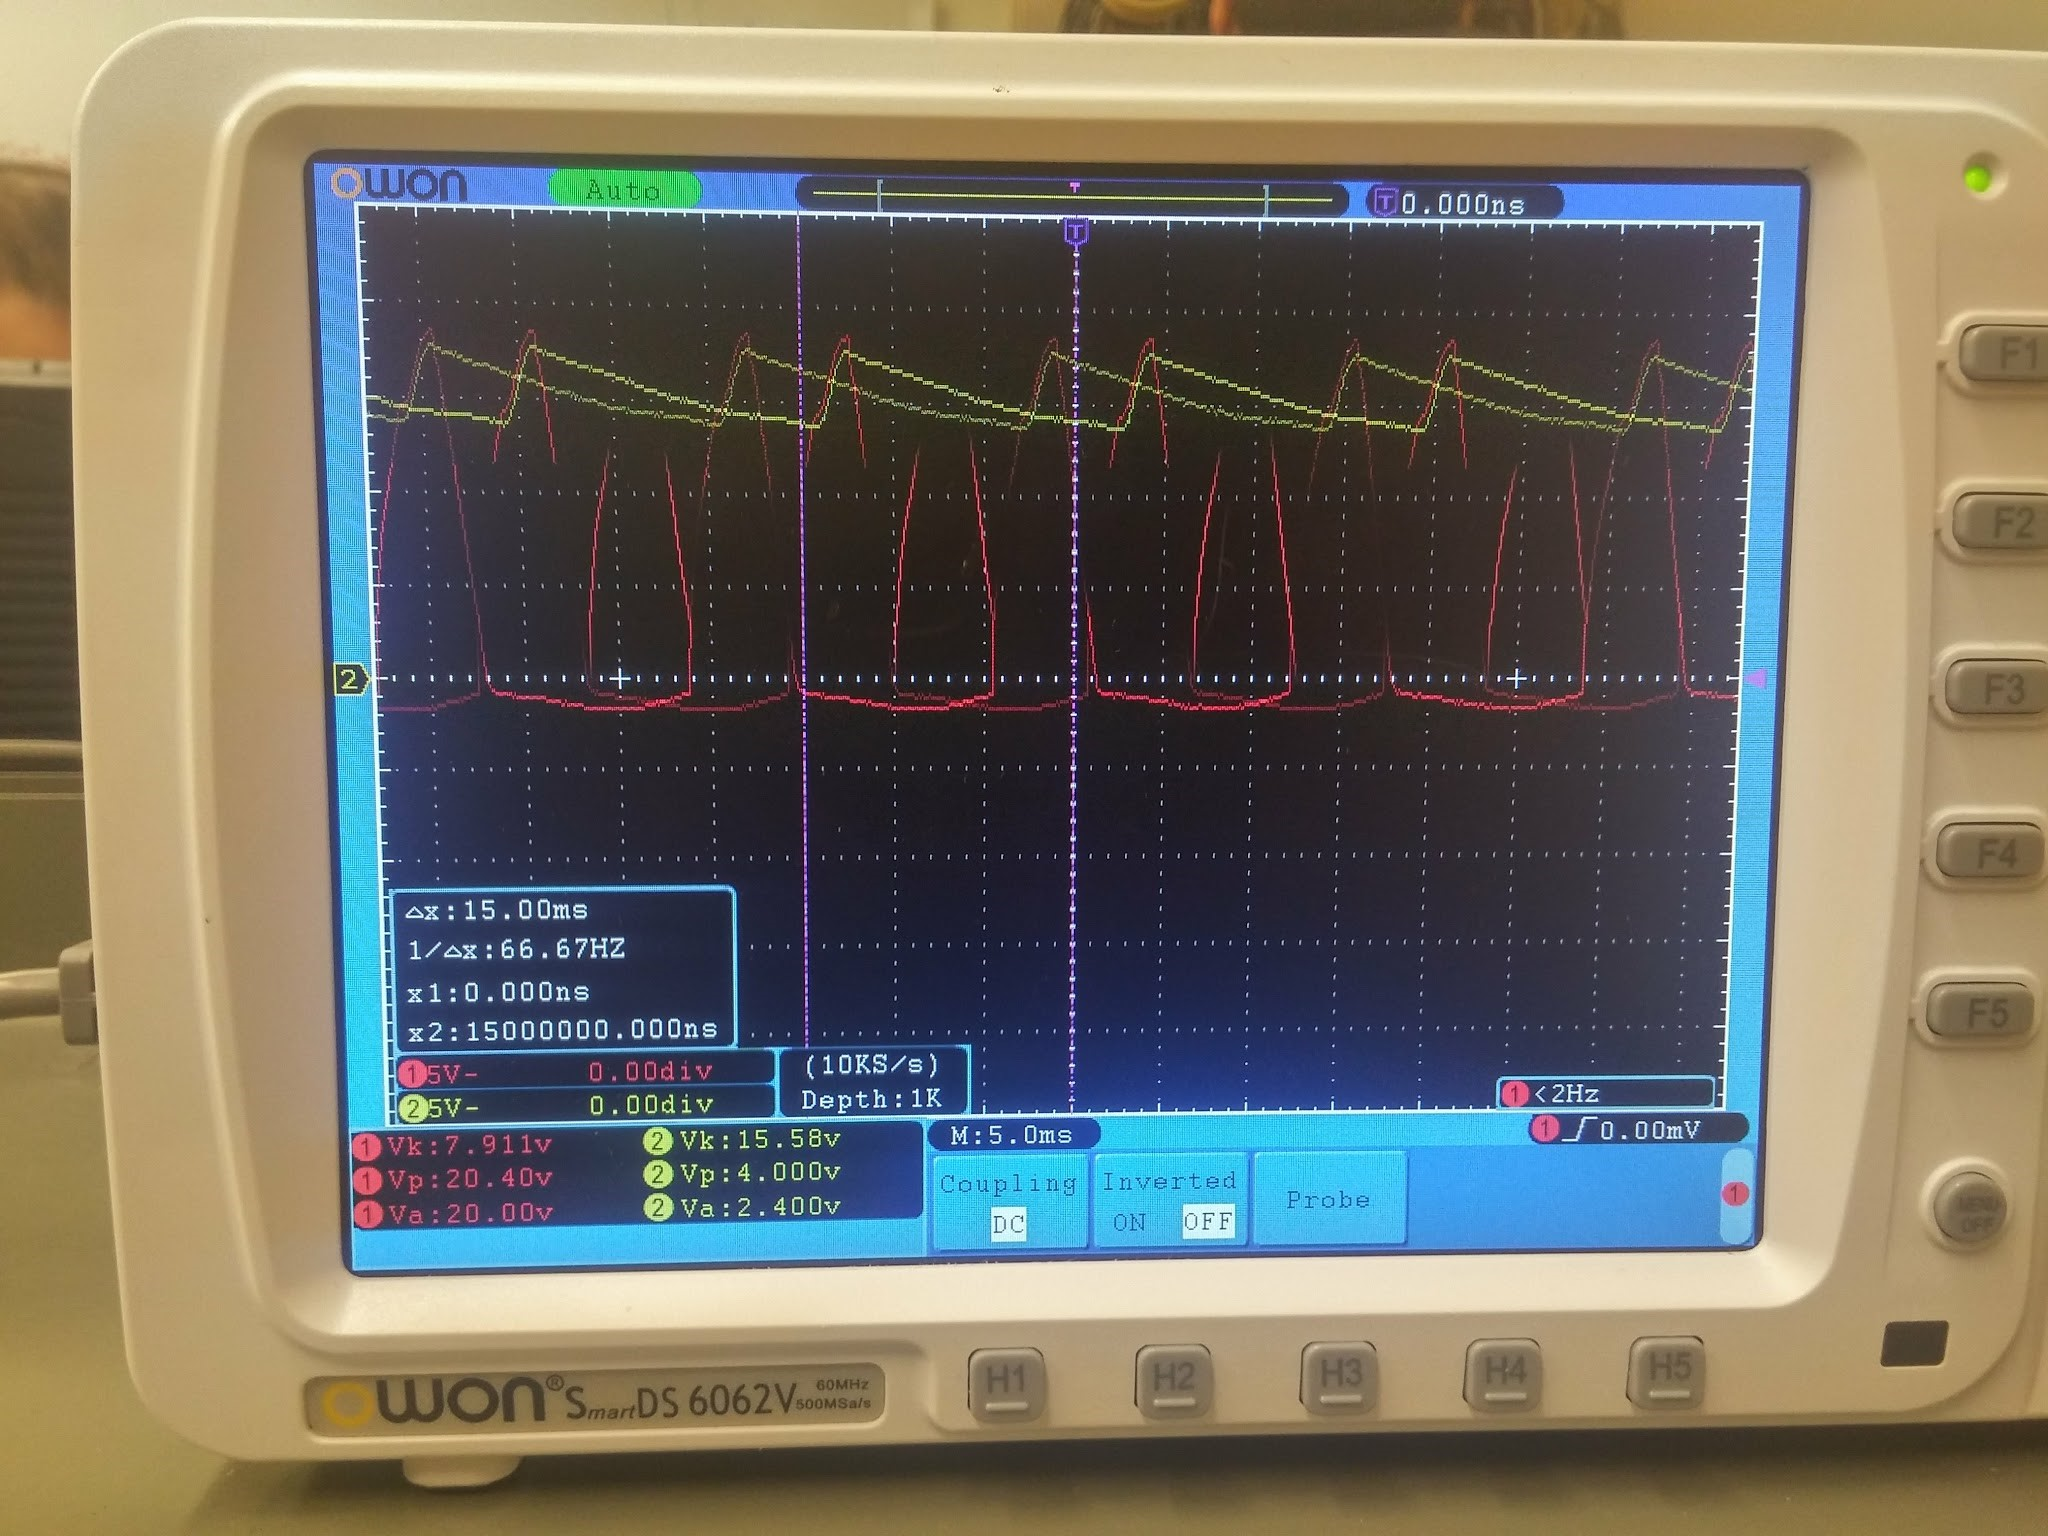
\includegraphics[width=\columnwidth]{Res200Cap100.eps}
	\caption{Input and Output of our filter capacitor circuit with a
	200$\Omega F$ resistor, and a 100$\mu F$ capacitor.}
	\end{figure}
	
	\begin{figure}[H]
	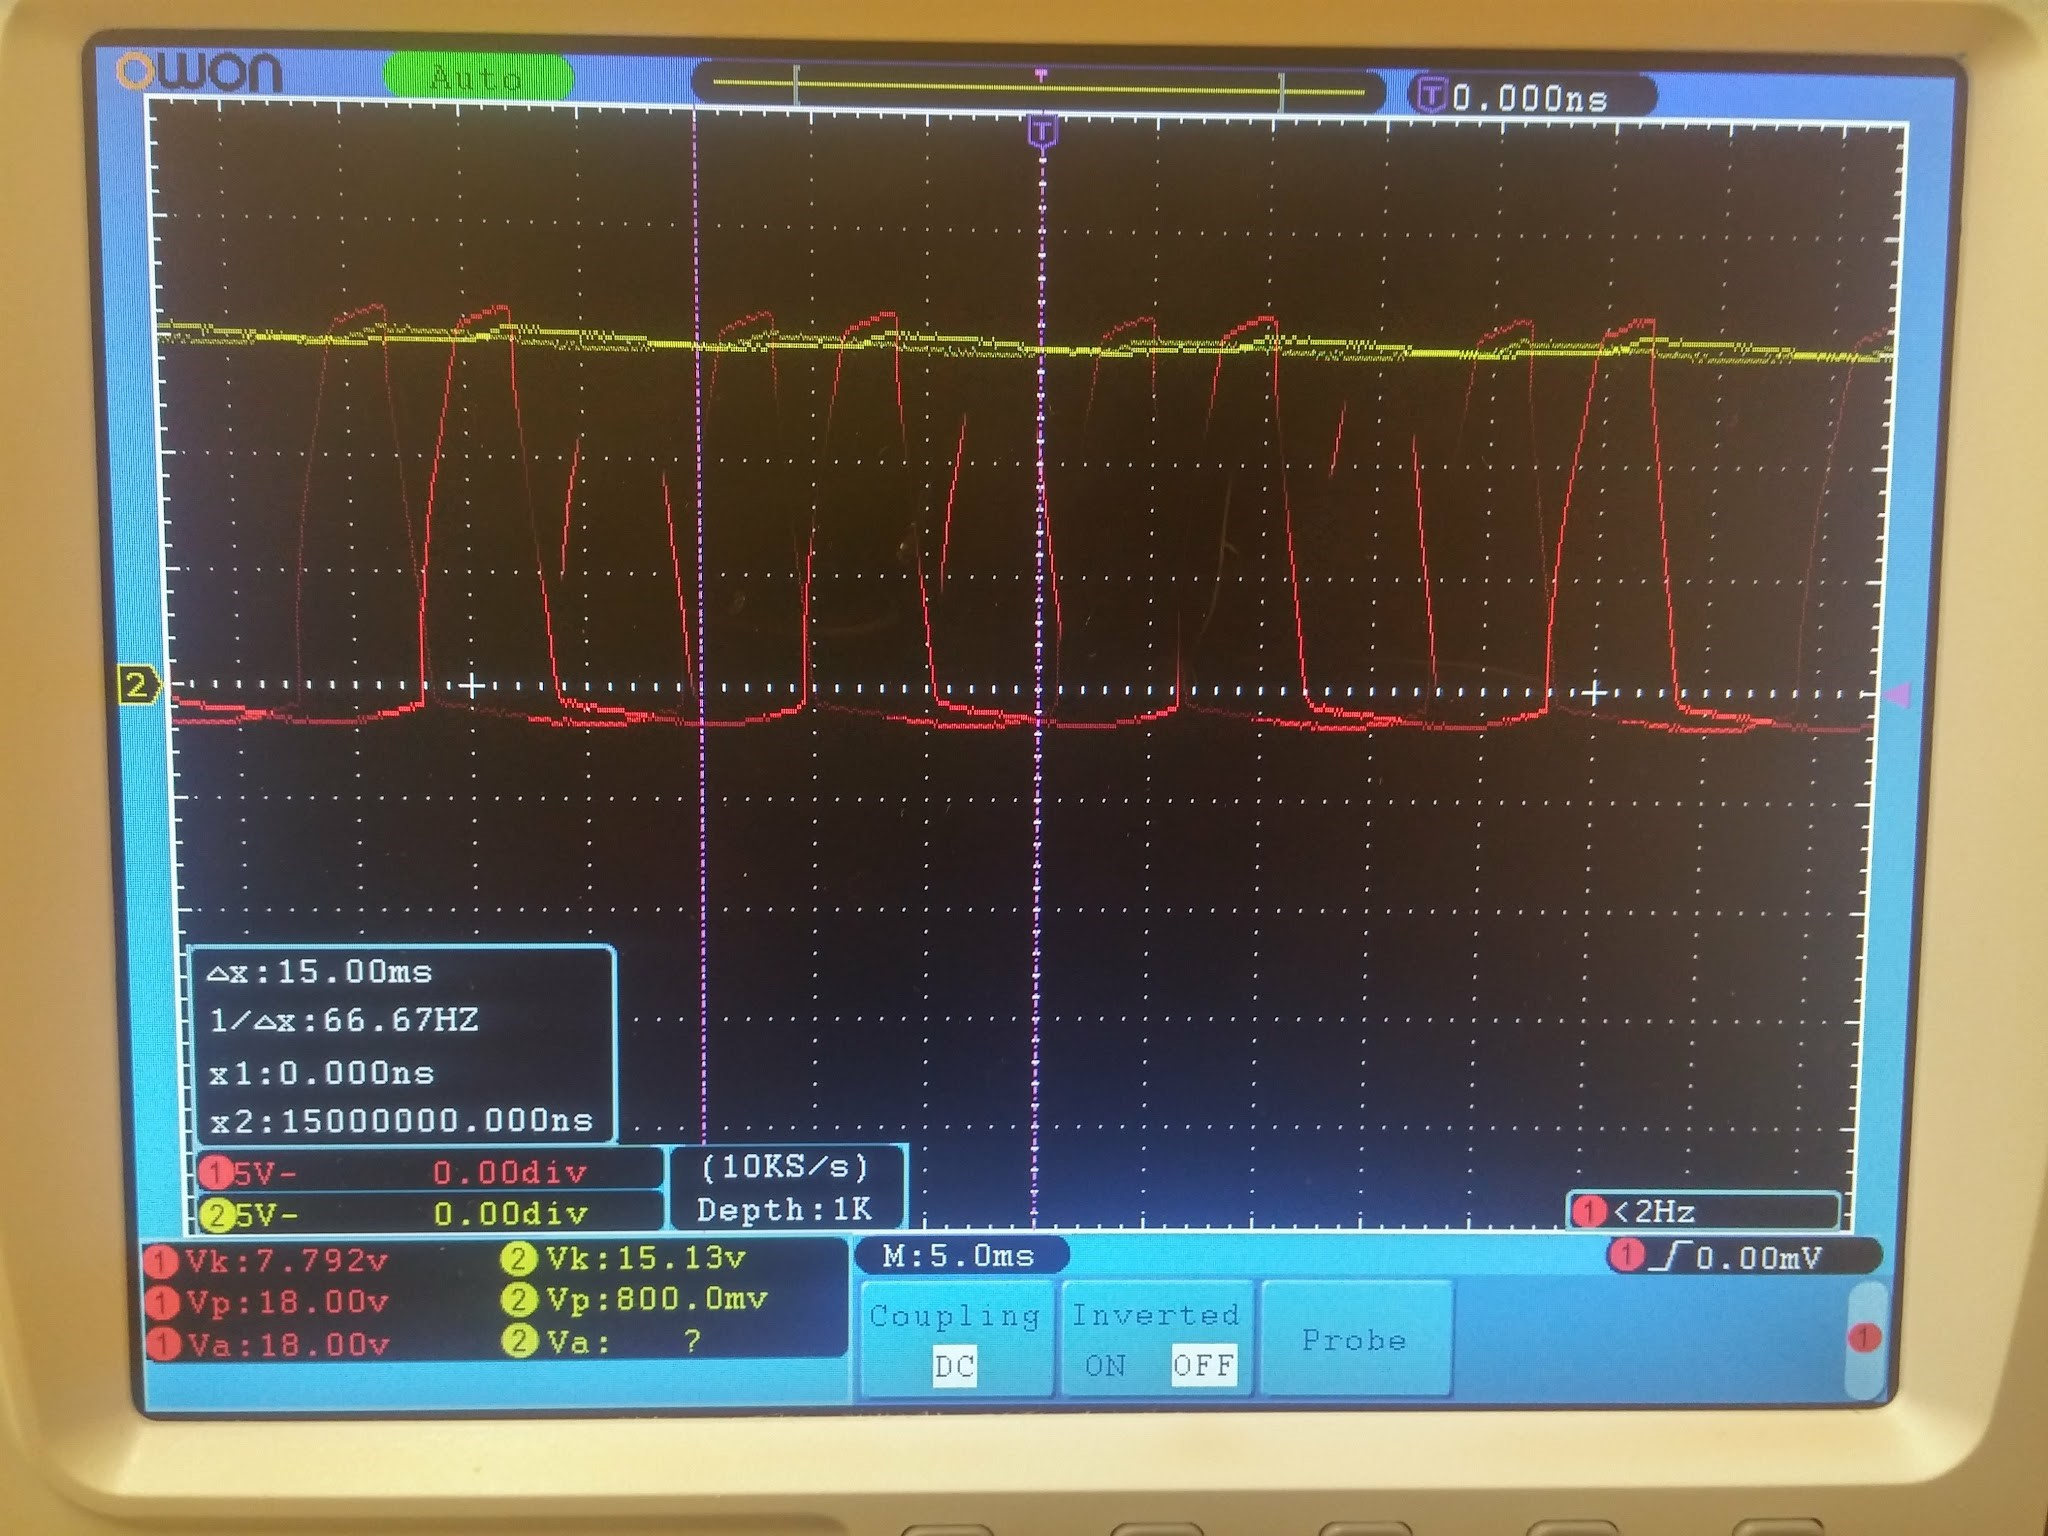
\includegraphics[width=\columnwidth]{Res200Cap1000.eps}
	\caption{Input and Output of our filter capacitor circuit with a
	200$\Omega F$ resistor, and a 1000$\mu F$ capacitor.}
	\end{figure}
	
	\begin{figure}[H]
	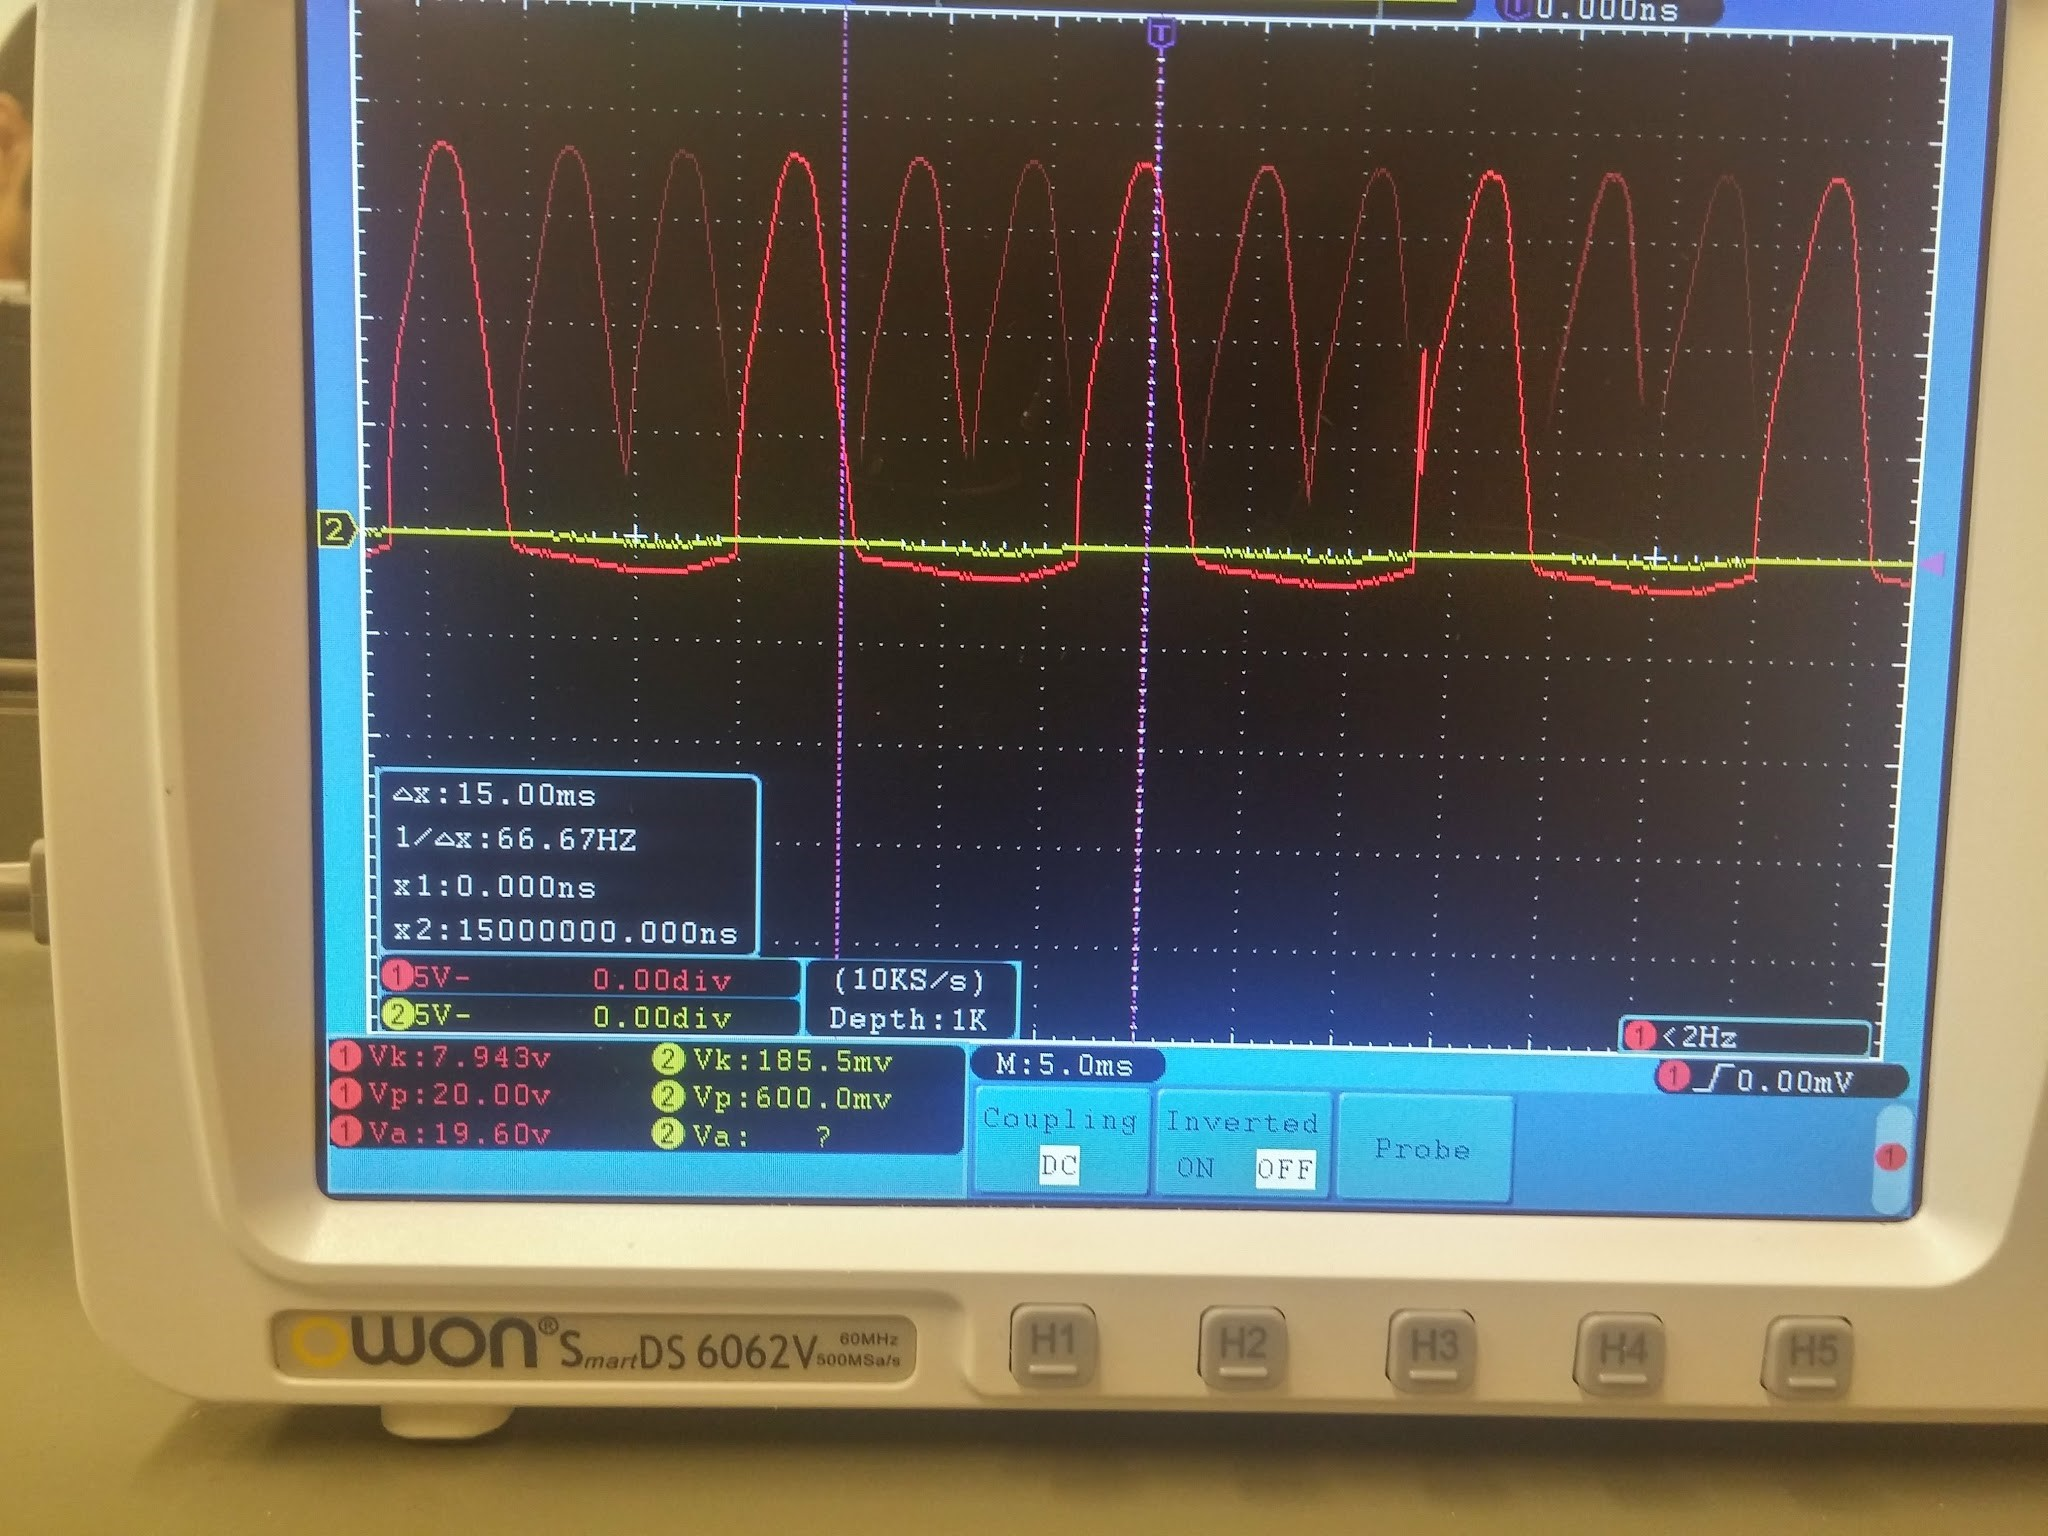
\includegraphics[width=\columnwidth]{Res1kCap10.eps}
	\caption{Input and Output of our filter capacitor circuit with a
	1k$\Omega F$ resistor, and a 10$\mu F$ capacitor.}
	\end{figure}
	
	\begin{figure}[H]
	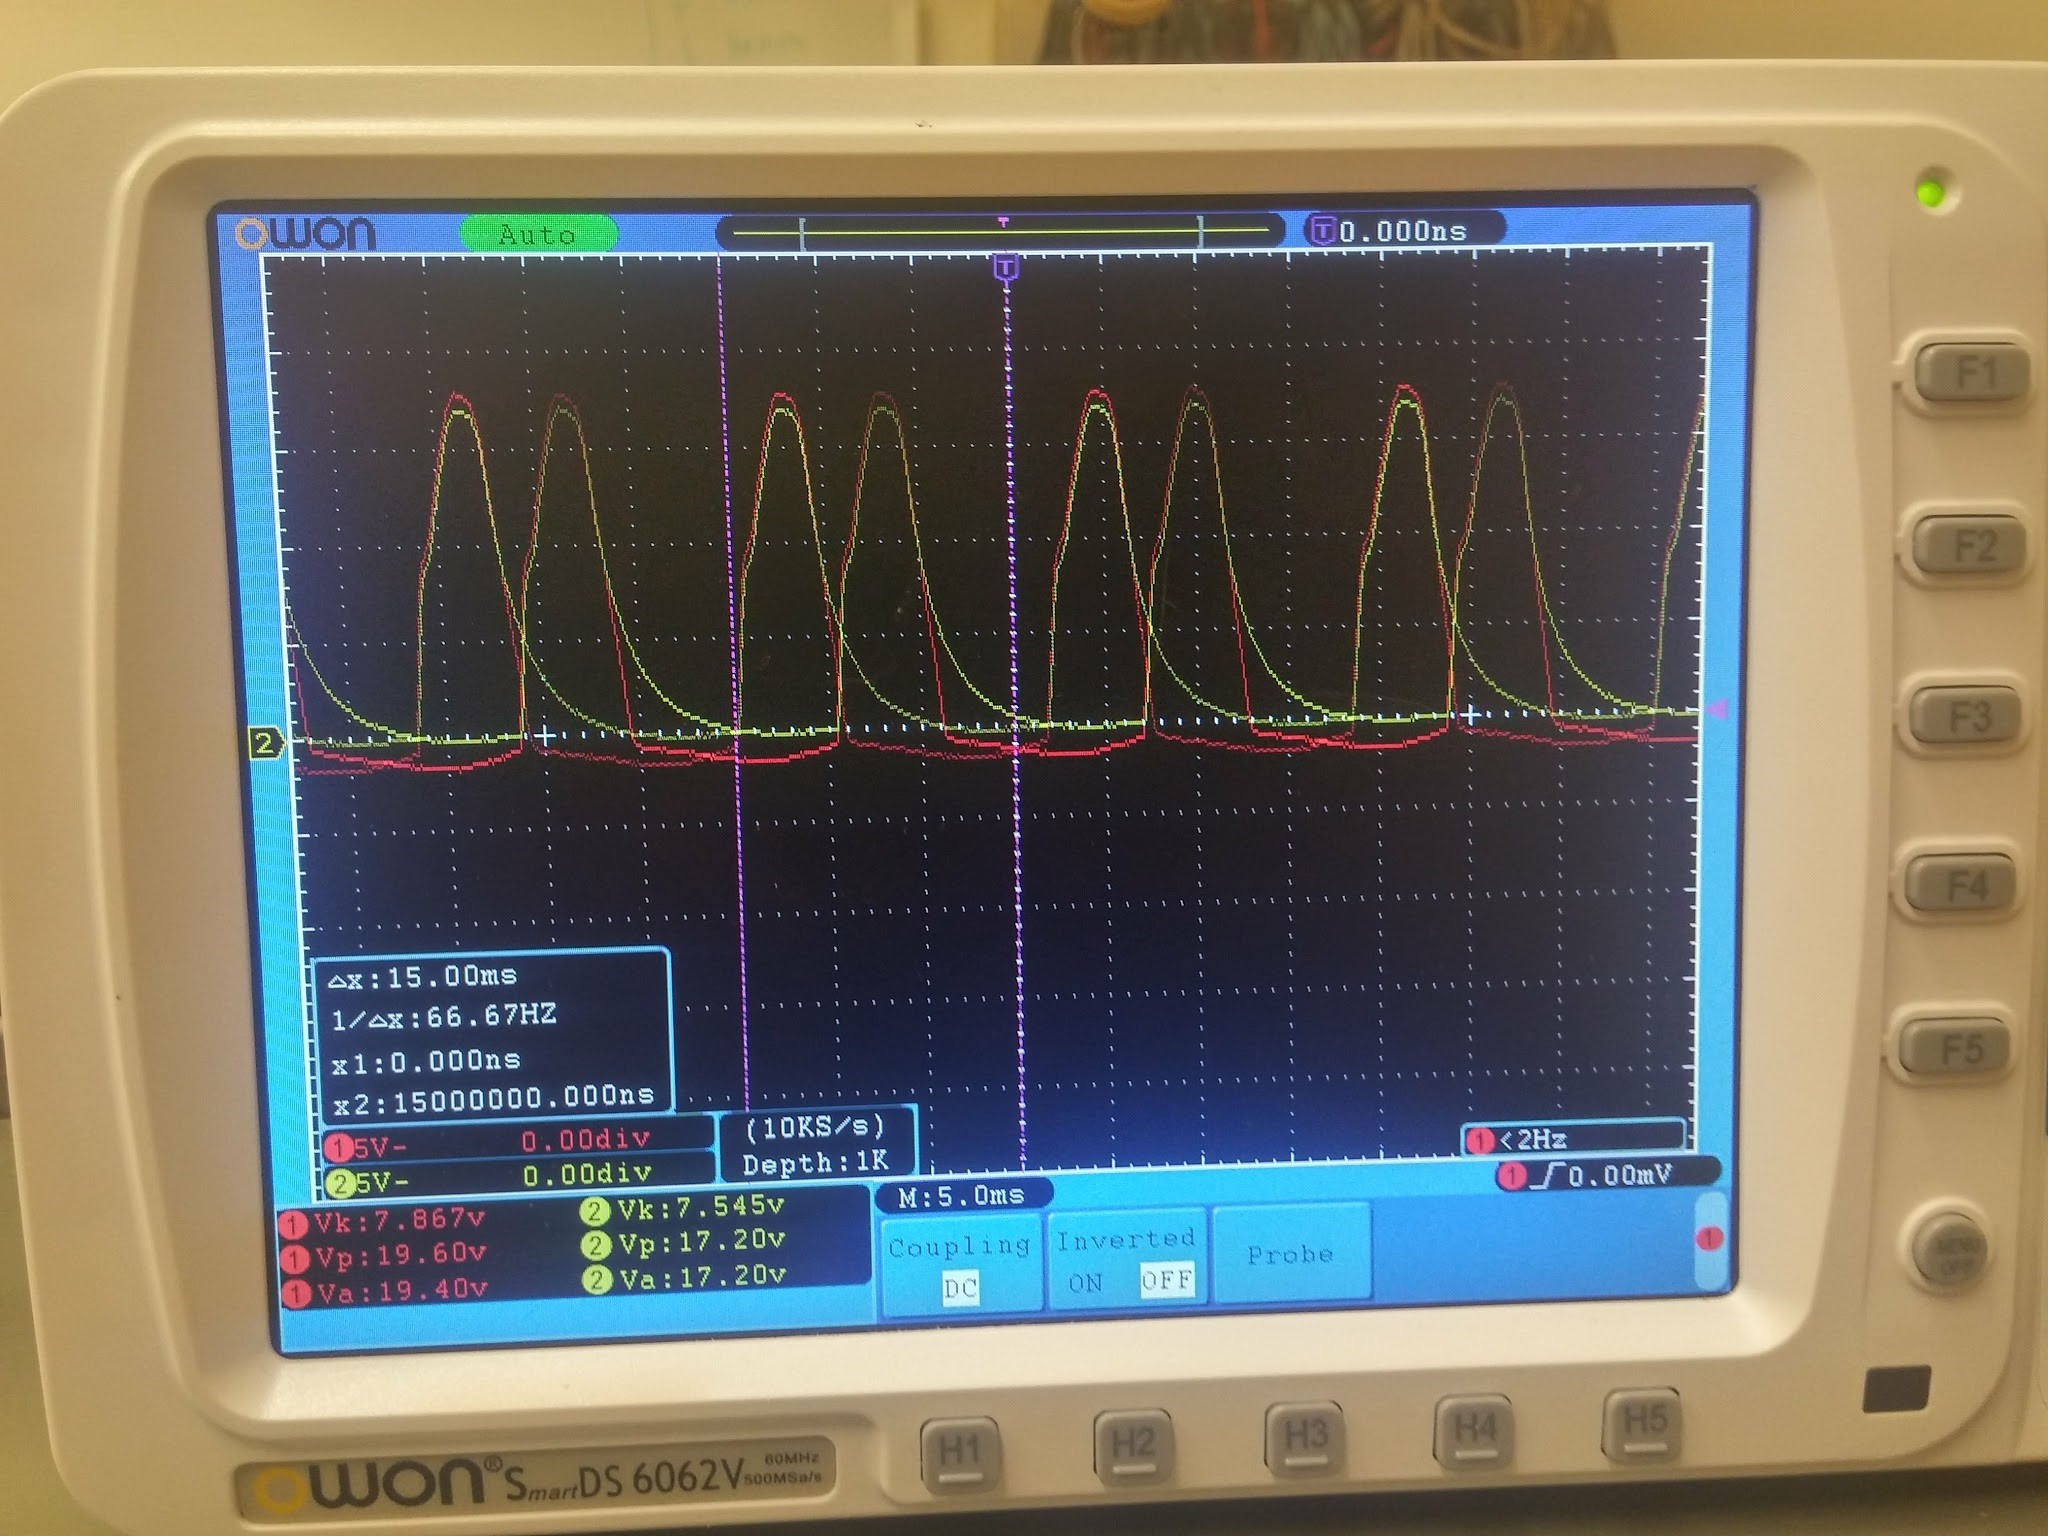
\includegraphics[width=\columnwidth]{Res1kCap100.eps}
	\caption{Input and Output of our filter capacitor circuit with a
	1k$\Omega F$ resistor, and a 100$\mu F$ capacitor.}
	\end{figure}
	
	\begin{figure}[H]
	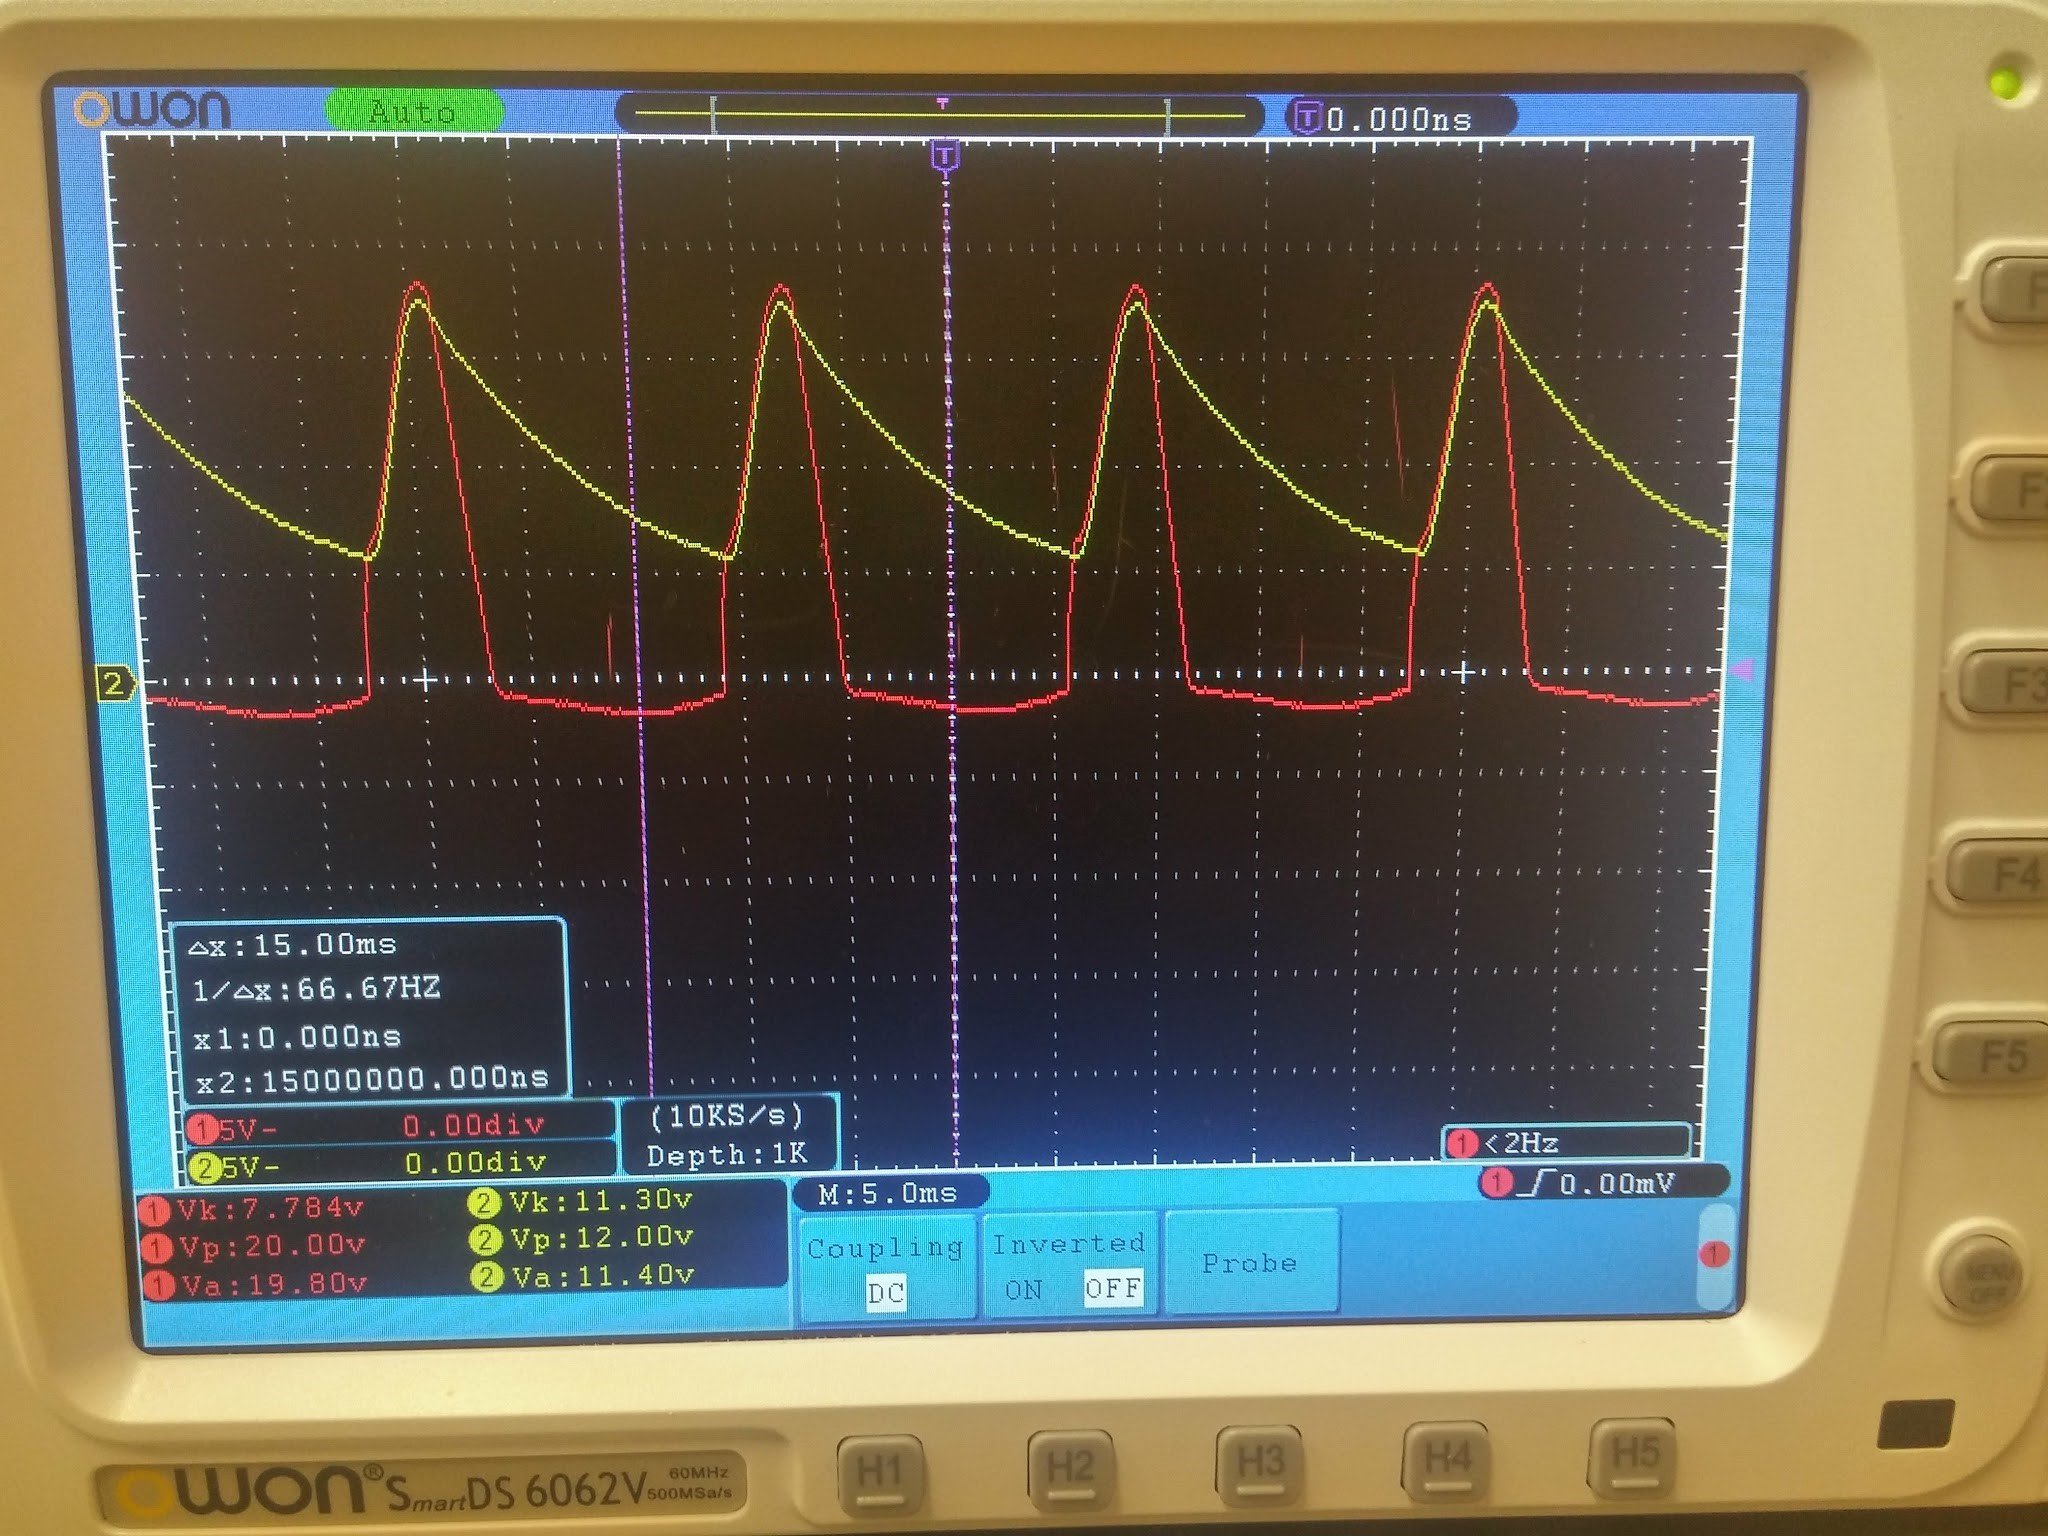
\includegraphics[width=\columnwidth]{Res1kCap1000.eps}
	\caption{Input and Output of our filter capacitor circuit with a
	1k$\Omega F$ resistor, and a 1000$\mu F$ capacitor.}
	\end{figure}
	
	\subsection{3-7: Voltage Regulators}
	
	\begin{figure}[H]
	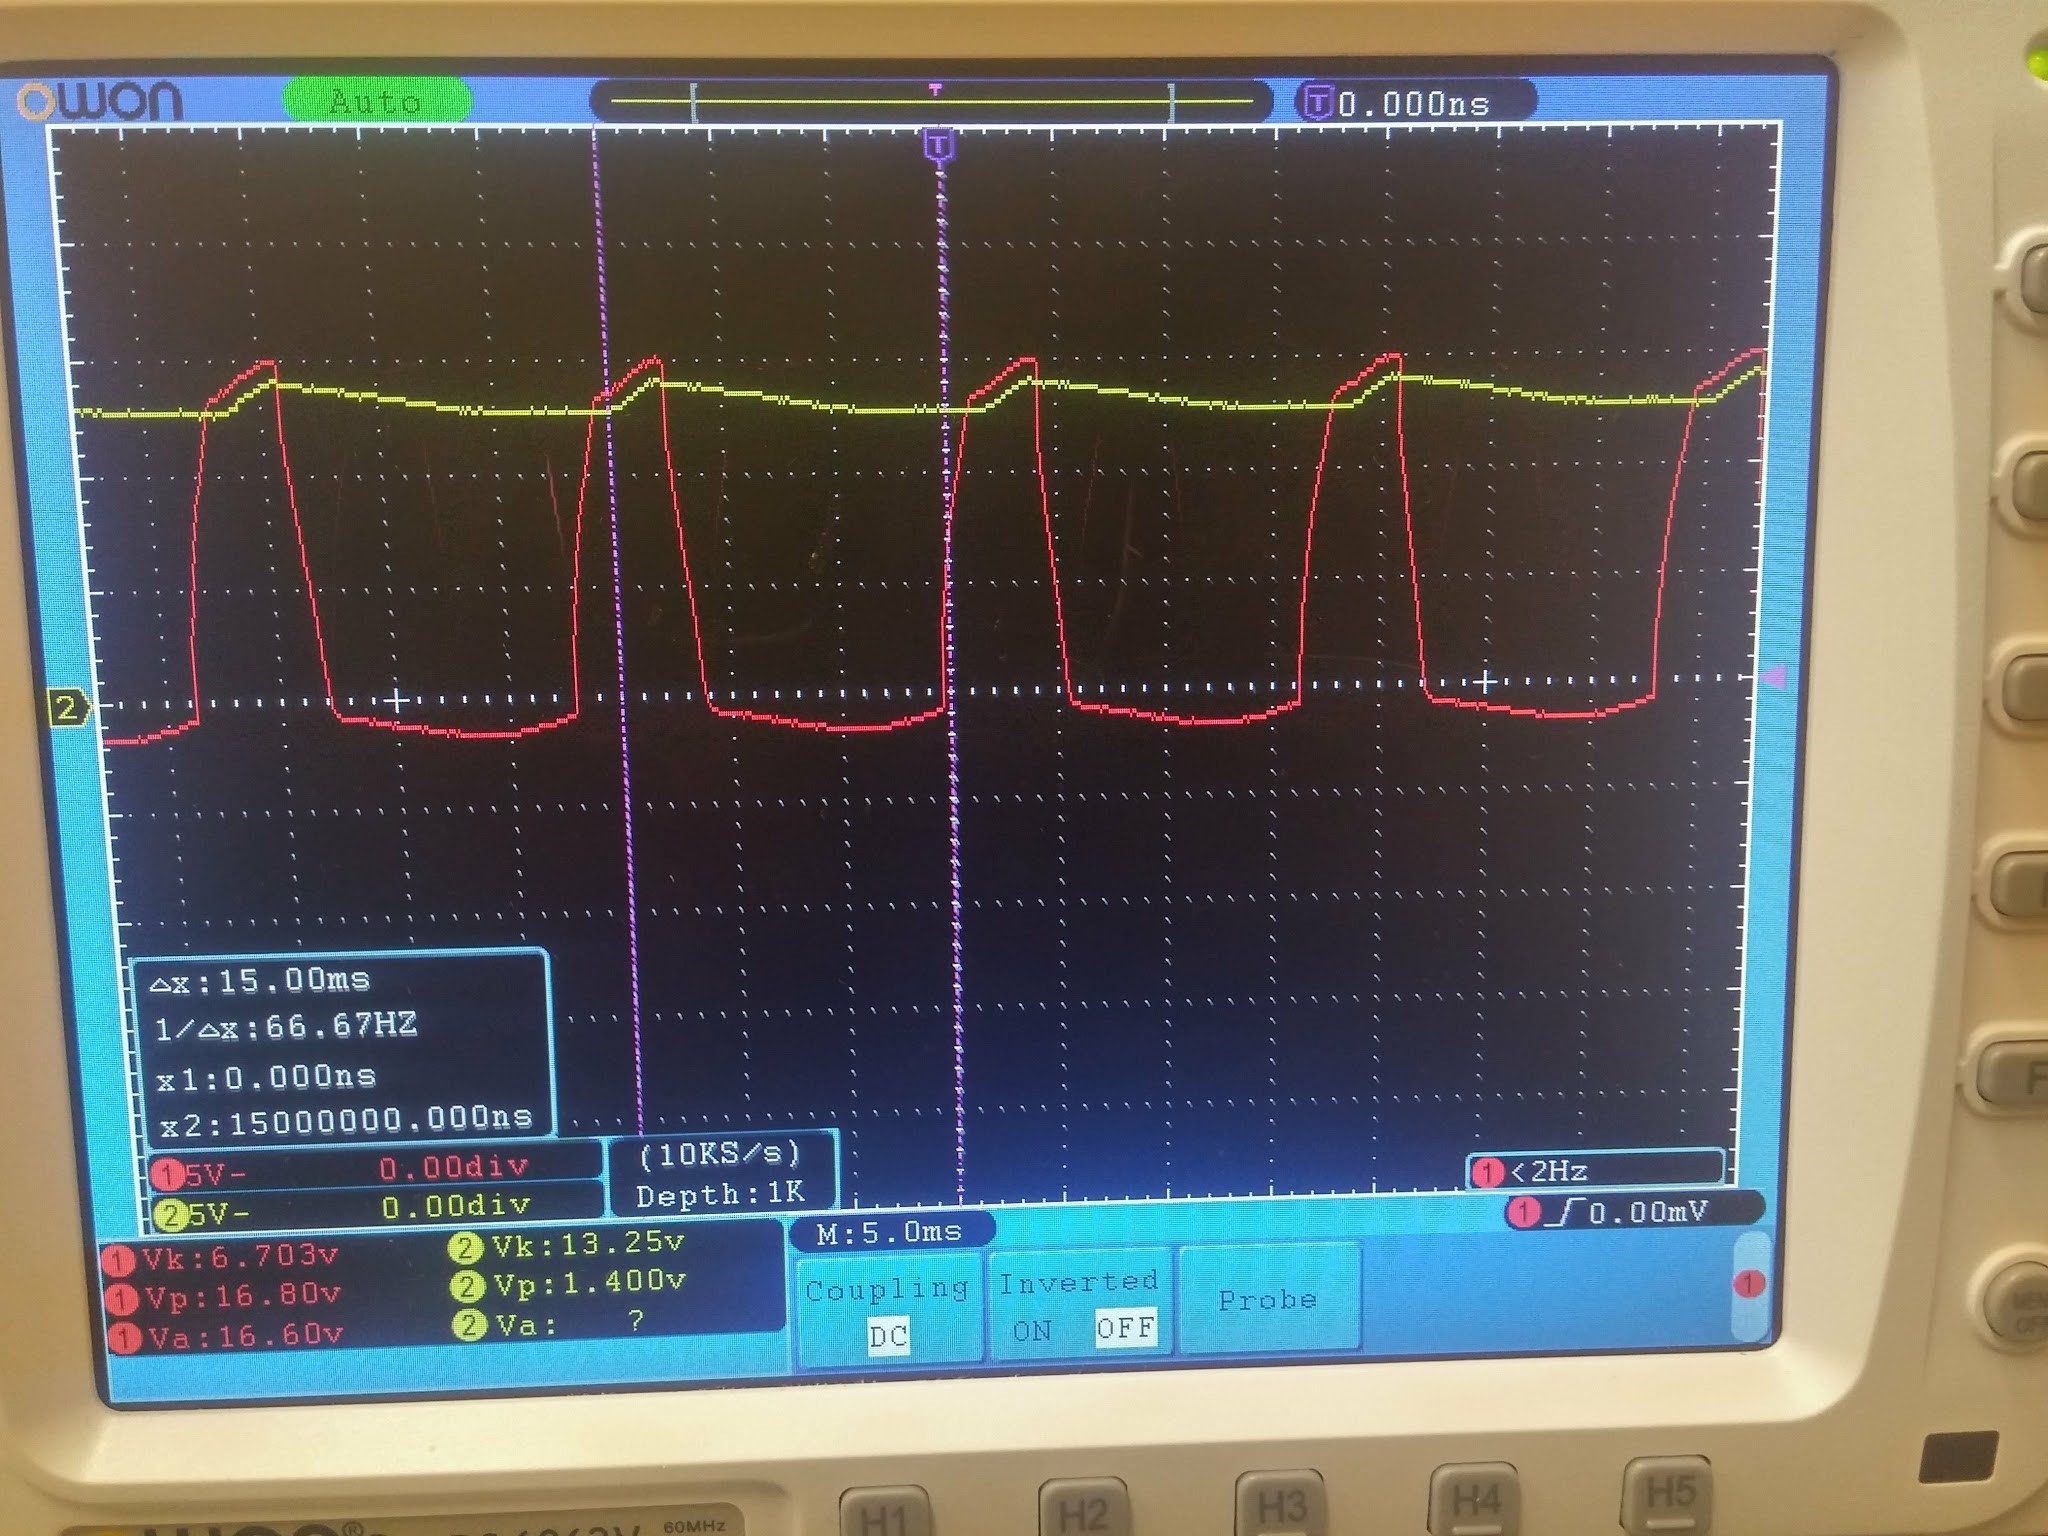
\includegraphics[width=\columnwidth]{Res1kCap1000VoltReg.eps}
	\caption{Input and Output of our voltage regulator circuit with a
	1k$\Omega F$ resistor, and a 1000$\mu F$ capacitor.}
	\end{figure}	
	
\section{Discussion}
	
	\subsection{3-1: Transformer Output Voltage Measurements}
	
	The purpose of this experiment was to show you how much percentage of the full output you get
	when grounding the full width of the circuit, versus going from center tap to ground.
	Theoretically, if your center tap is directly in the middle of your secondary winding, then our
	output voltage should be half of what it would be if you connected your circuit across the whole
	secondary wiring.
	
	The precision of these transformers is never going to be 100\% accurate without a financial
	burden being introduced, so for our experiment, we see that our center tap is close enough
	to half the output voltage of the full voltage of the transformer.

	\subsection{3-2: Diodes}
	
	We do see a small ohmic effect when it comes to our diode. There is a small voltage drop across
	the diode, but it is a (depending on your input voltage) negligible amount.
	
	For which side is the anode, and which side is the cathode, by definition, the Anode is the side
	that current comes in from an outside source, where as the Cathode is the side that outputs current.
	The cathode side is generally marked with a thin band on the diode that is a different color from the
	rest of the diode.
	
	\subsection{3-3: Half-Wave Rectified Power Supply}
	
	We find out in a later homework assignment how a P-N junction works, but the consequences of
	such are seen here. We see from our image that all of our negative voltage is blocked by diode.
	This is a forward bias. Due to the depletion layer that is formed when we send a negative voltage
	through the diode, our output for the negative part of our input voltage goes to zero.
	
	When we connect the diode in a reverse bias, we end up with an opposite effect. All of our positive
	voltage now gets blocked by the diode, and our negative voltage is able to go through.
	
	\subsection{3-4: Full-Wave Rectified}
	
	For experiment 3-4, the full-wave rectifier gives our circuit 2 options. Since we are using the 
	center tap as ground, and forward biasing both of our diodes, what we should see for Channel 1
	is a sinusoidal wave that has half the voltage of the full output of our transformer. What we get
	for Channel 2 though, is that since both sides of the transformer are outputting a voltage, with
	the center tap as ground, and both of the diodes are forward biased, we are getting only the 
	positive voltages from both "`sources"', giving us what looks like the absolute value of a 
	sinusoidal wave.
	
	\subsection{3-5: Bridge Rectifier}
	
	The bridge rectifier configuration is very similar to our full-wave rectifier, but we have
	two extra diodes in place to keep the negative voltage from passing through to our other 
	side of our parallel circuit and causing a short.
	
	This allows to have a full-wave rectifier, without the cost of losing half of our voltage due
	to having to use the center tap. The benefit of this is that our amplitude will be twice as 
	high as the full-wave, and the same as the half-wave, but the RMS for our bridge rectifier
	will be twice as high as our RMS for our half-wave. 
		
	\subsection{3-6: Filter Capacitors}
	
	With experiment 3-6, we replaced the 10k$\Omega$ resistor with a RC parallel circuit. What
	we saw with the output was a filtered voltage output. Since we are getting the same bridge
	rectifier in place, we are only seeing positive voltages, ranging from 0V to our peak of 20V,
	but this time around, we have a capacitor in series with our resistor for the ground. 
	
	We know that the capacitor has a capacitive reactance that is represented as
	$X_C = \frac{1}{\omega C}$, so the higher our capacitance, the lower our capacitive reactance,
	and thus, the lower our impedance. Also, the lower our resistance, the lower our impedance as
	well. This would explain why we have the most stable output with the combination of 200$\Omega$
	resistor and a 1000$\mu F$ capacitor, as this configuration will give us the lowest impedance. 
	
	\subsection{3-7: Voltage Regulators}
	
	We saw a more stable DC voltage for our output voltage in the voltage regulator circuit. Since 
	a voltage regulator is designed to maintain a constant voltage level, we see less of a drop in 
	voltage when our input voltage drops as the voltage is a function of frequency.

\section{Conclusion}

With using diodes, capacitors, and resistors, we are able to show how we can take an AC volatage
source, and modify it to our needs, slowly but surely with each experiment. We first show how to 
filter out certain polarities of voltages, then how to not lose our "`filtered"' voltages with our
full-wave rectifier. Next we learned that by not connecting to the center tap, but adding more diodes
in, we can avoid losing half of our amplitude. Then, using filter capacitors and voltage regulators, we
can smooth out our AC input into a DC output.

Is this how our Elenco Variable Power supply works? Though we may complain about the lack of granularity
and precision at lower voltages, when you add the overhead complexity of a potentiometer and that they
are getting an AC input, and how difficult it was for us to smooth out our AC input into a flat DC
output, you can really appreciate how hard something that we presumes should be so "`easy"' is. 

Every lab is here to teach us that nothing is easy nor comes for free in physics. Granularity costs
time, money, and knowledge. As does precision, and as physicists if we feel we can do better, we 
should, instead of simply saying so.

\end{document}